% !TEX root = manuscrit.tex
	
Since this protocol is parameterized by the ring size $n$, 
model-checking does not permit to verify whether it is valid for all
values of $n$. Therefore, while automated verification was used to
prove the required properties for small values of $n$, we provide an
inductive proof to obtain the correctness for arbitrary values of $n$
in the asynchronous model.

%Synth:  we prove by induction that the mechanically generated algorithm is also correct for any ring size except when an impossibility result holds (that is, when the number of robots divides the ring size). Our method can be seen as a first step towards  ``correct by design'' actual robot protocol implementations. 


	\section{Correctness of the new algorithm }
\label{subsec:induction}  

We first prove point \emph{(c)}: the exploration is performed
by cycling within the legitimate configurations and point \emph{(b)}:
from all non-legitimate configurations a legitimate configuration is
reached.
%\todo{rappeler la reference de la def contenant les types (like $A$, $B$ or $L1$)}

\begin{definition}
\label{note:type}
We note $[Type^n(x, y, z), \ \varphi(x, y, z)]$ the set of
configurations such that $Type$ is the type of the configuration, $x$, $y$ and $z$ correspond to the number of free
nodes that isolate each robot from the other, and $\varphi(x, y, z)$ is
an additional constraint restricting the scope of values for $x, y, z$.
\end{definition}
Recall that $n = x+y+z+3$ remains constant, with $n\geq
10$. Constraints defining the type itself are omitted, for instance, 
$[B^n(x, y, x) \mid x\neq y \wedge $ $x> 0$ $\wedge \ n = y+2x+3]$ is
simply denoted by $[B^n(x, y, x)]$.



\begin{definition}
\label{note:state}
The tuple $(s_x, s_y, s_z, [\textit{Type}^n(x, y, z), \varphi(x, y, z)])$ denotes
the set $$\{(s_x, s_y, s_z, c) \mid c \in [\textit{Type}^n(x, y, z), 
\varphi(x, y, z)] \}$$ of system states, where $s_x$ (respectively $s_y$, 
$s_z$) is the local state of the robot positioned before the
$x$ (respectively $y$, $z$) free nodes.\\
For $w \in \{x, y, z\}$, state $s_w$ belongs to $\Front$, $\Back$, 
$\RLC$. For the sake of readability, we do not
represent $\textit{Idle}$ states, hence only scheduler choices about robots
that can move are seen.

For a set $P$ of system states, we denote by $\mathcal{C}(P)$ the set
of configurations of $P$ and by $\mathcal{R}(P)$ the set of rules of
the algorithm that can be applied on $P$. For a rule $R \in
\mathcal{R}(P)$, we define: $$succ_{R}(P)=\{s' \ | \ s \xrightarrow{R}
s' \textrm{ for some } s \in P\}$$ the set of states produced by
applying $R$ to states of $P$.
\end{definition}

%\todo{ref def 13}

An abstract view of the algorithm is shown in Figures~\ref{fig:all}
and~\ref{fig:lower} using these notations. Gray states are
initial states, more particularly the light gray ones are legitimate states.  Each
$\textit{Move}$ transition is guarded by a condition between brackets
and corresponds to the choice of the scheduler to let all robots
move. In the $\textit{Move}_{any}$ transition, the scheduler lets only
a single robot move.


\begin{figure}[htbp]
\centering
%\input{algomin.tex}
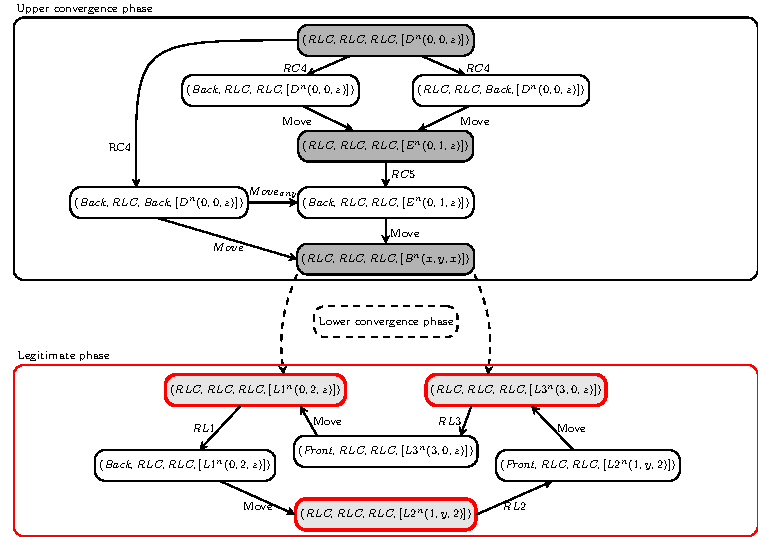
\includegraphics[scale=1.2]{figures/figALgoMin2}
\caption{Graph of Min-algorithm.}
 \label{fig:all}
\end{figure}

\begin{figure}[htbp]
\centering
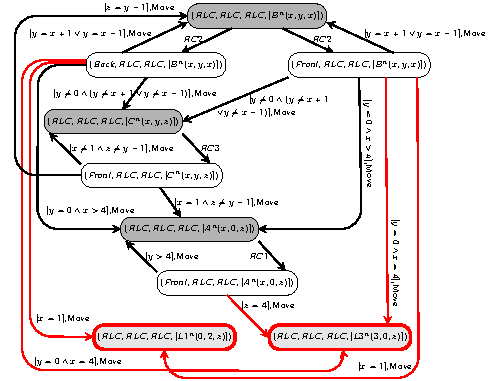
\includegraphics[scale=2]{figures/figlowerP}
\caption{Lower convergence phase.}
 \label{fig:lower}
\end{figure}

\subsubsection{Exploration from legitimate configurations}

We prove the following theorem:
\begin{theorem}
\label{th:legit}
From any legitimate configuration the ring (of size $n \geq 10$, 
co-prime with $3$) is perpetually explored.
\end{theorem}

\begin{figure}[bt] 
\centering
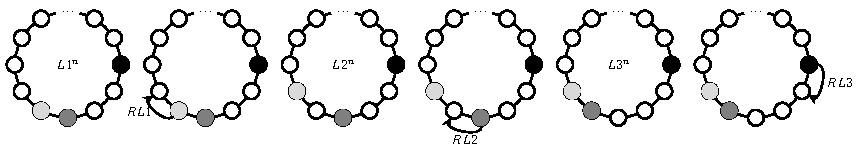
\includegraphics[scale=1]{figures/figLegit}
\caption{A step for the exploration.} 
\label{fig:Legit} 
\end{figure} 

The result holds if from a legitimate configuration ($L1, L2, L3$) only
legitimate configurations are reached, and if from any legitimate
configuration, an identical configuration is reached, where all
positions have been shifted $p$ times to the same direction, for any
$p\in\N$. In particular, when $p>0$ is a multiple of $n$, all robots
have visited all nodes.
These two properties are expressed by the following \textsf{LTL} formulas:\\

\begin{enumerate}[parsep=0cm, itemsep=0cm, topsep=0cm]
\item %\begin{lemma} 
\noindent \label{lem:GL}$\G \ (\mathbb{L} \Rightarrow \G \ \mathbb{L})$\\
%\end{lemma}
\item %\begin{lemma}
\label{lem:explor}$\forall i, m = 1, 2, 3$, $\forall j \in
  \{0, 1, \ldots, n-1\}$, $\forall p \in \mathbb{N}$, \\
  $\G (Lm \wedge r[j]=r_i \Rightarrow \F (Lm \wedge r[j+p]=r_i))$\\
%\end{lemma}
\end{enumerate}

  where $Lm$ is the predicate indicating that the configuration
  belongs to the corresponding set and $r[j]= r_i$ is the binary
  predicate giving the absolute position $j$ for robot $r_i$.

By construction and for all $n\geq 10$, the first formula is satisfied
since the only possible moves from $L1$, $L2$ and $L3$
for scheduled robots not staying idle are: \\\smallskip
\small{%%%%%%%%%%%%%%%%%%%%%%%%%%here%%%%%%%%%%%%%%%%%%%%%%%%%%%%%r                                                                                                                                                                                                                                                                                                                                                                                                                                                                                                                                                                                                                                                                                                                                                                                                                                                                                                                                                                                                                                                                                                                                                                                                                                                                                                                                                                                                                                                                                                     
\noindent
$succ_{RL1}~((\RLC, \RLC, \RLC, [L1^n(0, 2, n-5)]))$
$ = (\Back, \RLC, \RLC, [L1^n(0, 2, n-5)]), $\\ \smallskip
$ succ_{Move} (( \Back, \RLC, \RLC, [L1^n(0, 2, n-5)]))$ 
$= (\RLC, \RLC, \RLC, [L2^n(1, 2, n-6)]), $

\medskip \noindent
$succ_{RL2}~(( \RLC, \RLC, \RLC, [L2^n(1, 2, n-6)]))$
$ = (\RLC, \Front, \RLC, [L2^n(1, 2, n-6)]), $\\\smallskip
$succ_{Move} ((\RLC, \Front, \RLC, [L2^n(1, 2, n-6)]))$
$= (\RLC, \RLC, $ $\RLC, [L3^n(0, 3, n-6)]), $

\medskip \noindent
$succ_{RL3}~(( \RLC, \RLC, \RLC, [L3^n(0, 3, n-6)]))$
$ = (\RLC, \RLC, \Front, [L3^n(0, 3, n-6)]), $\\\smallskip
$succ_{Move} ((\RLC, \RLC, \Front, [L3^n(0, 3, n-6)]))$
$ = (\RLC, \RLC, \RLC, [L1^n(0, 2, n-5)]).$\\}

As mentioned previously, the second formula ensures the perpetual
exploration.  The proof is an easy induction over $p$, for an
arbitrary size $n$.

The base case for $p=1$:  $(Lk \wedge r[j]=r_i) \implies \F (Lk \wedge r[j+1]=r_i)$ 
results from chaining the three moves described above, 
as illustrated in Figure~\ref{fig:Legit}. For
the induction step, assume that the property holds for $p$.  This
implies: $$(Lk \wedge r[j]=r_i) \implies \F (Lk \wedge r[j+p]=r_i).$$
Setting $j'= j+p$ and
using the base case $(Lk \wedge r[j]=r_i) \implies \F (Lk \wedge r[j+1]=r_i)$, 
we obtain: $(Lk \wedge r[j']=r_i) \Rightarrow \F
(Lk \wedge r[j'+1]=r_i)$.\\Hence,  $(Lk \wedge r[j]=r_i) \Rightarrow \F (Lk
\wedge r[j+p+1] = r_i)$ 
and the property holds for $p+1$.


\subsubsection{Convergence from illegitimate configurations}

\begin{theorem}\label{th:conv}
  From any non legitimate configuration, a legitimate configuration is
  eventually reached (for a ring of size $n \geq 10$, co-prime with
  $3$).
\end{theorem}

To establish the convergence result, we associate with any subset $P$
of system states a tree $\T(P)$ rooted in $P$, with nodes the subsets
of states obtained by applying the rules of the algorithm.  Reaching a
set of successors in $\mathbb{L}$ without pending moves results in a
leaf.  More precisely:
\begin{definition}
\label{def:conv}
Given the set $\mathcal{R}$ of rules of the \emph{Min-Algorithm}, 
let $P_0$ be a subset of system states. The tree $\T(P_0)$ has
$P_0$ as root and for each node $P$:
\begin{itemize}
\item If $\mathcal{C}(P) \subseteq \mathbb{L}$ and for all $s \in P$, 
  $w \in \{x, y, z\}$, $s_w \notin \{\Front, Back \}$, then the node has
  no successor.
\item Otherwise the node $P$ has a successor $succ_{R}(P)$ for each $R
  \in \mathcal{R}(P)$.
\end{itemize}
\end{definition}

We now prove that for any set of states $P$ such that $\mathcal{C}(P)$
is contained in one of the non legitimate configurations types, the
tree $\T(P)$ is finite. This yields the desired convergence proof. If
for some $P$, the tree $\T(P)$ is infinite, then there exists an
infinite sequence of rules (on an infinite path of this tree) such
that for all successor sets $P'$ of $P$ along this sequence, either
$\mathcal{C}(P') \nsubseteq \mathbb{L}$ or there is some $s \in P'$
such that $s_w \in \{\Front, Back\}$ for some $w \in \{x, y, z\}$, 
meaning that the corresponding robot has a pending move.


To prove this result, we exhaustively verify the property for all
types $A^n$, $B^n$, $C^n$, $D^n$ or $E^n$, by inductive proofs, in
Lemmas~\ref{lemma:a} to~\ref{lemma:d} (where we assume $n \geq10$ and
$n$ co-prime with $3$). Note that  these lemmas must be proved in 
the order $A$, $C$, $B$, $E$ and $D$.
 Since $\mathbb{NL}^n = A^n \cup B^n \cup C^n
\cup D^n \cup E^n$ the result follows.
 

\begin{lemma}
\label{lemma:a}
The tree $\T(P)$ is finite for 
$P=(\RLC, \RLC, \RLC, 
[A^n(x, 0, z), 4 \leq x<z]).$
\end{lemma}
 
\begin{proof}
  The idea of the proof is as follows: recall that from an $A^n$
  configuration $(R_1, F_x, R_2, F_z)$ with $4 \leq x < z$, written
  $[A^n(x, 0, z), 4 \leq x<z]$, only one movement is feasible, leading to an
  $[L3^n(3, 0, z)]$ configuration if $x=4$ and to an $[A^n(x-1, 0, z+1)]$
  configuration otherwise.  Hence,  the number of free nodes in the $x$
  part decreases until an $L3$ configuration is reached.

  We first prove the property for an arbitrary $z$ when $x=4$ (base
  case). Then we prove the induction step on $x$.\\

%\begin{description}[parsep=0cm, itemsep=0cm, topsep=0cm]
\noindent \textbf{Base-case:} 
For $P=(\RLC, \RLC, \RLC, [A^n(4, 0, z)])$, with any $z \geq 6$,  the tree $\T(P)$ is finite
 with the moves:
\begin{center}
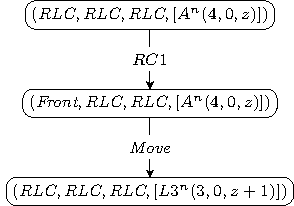
\includegraphics[scale=1]{figures/figAx4} 
\end{center}

\noindent \textbf{Induction step:} Assume that the tree
with root $P=(\RLC, \RLC, \RLC, [A^n(x, 0, z)])$, for any $z>x$ is
finite.
%when $n>10$ and $n, k$ are co-prime.
For $x+1 < z$, the moves are:
\begin{center}
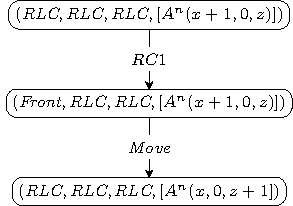
\includegraphics[scale=1]{figures/figA}
\end{center}
 they lead to $(\RLC, \RLC, \RLC, 
[A^n(x, 0, z+1])$ for which the tree is finite from the induction hypothesis. 
This ensures the desired result.
\end{proof}

\begin{lemma}
\label{lemma:c} The tree $\T(P)$ is finite for\\
$P=(\RLC, \RLC, \RLC, [C^n(x, y, z), 0<x<z<y])$
with $(x, z) \neq (1, 2).$
\end{lemma}

\begin{proof}
%A configuration $ c \in C^n$ is of the form: 
%$(R_1, F_x, R_1, F_y, R_1, F_z)$ with $0<x<z<y$.
  We first fix parameter $x$ and show that the tree for $P$ is
  finite, for any $y, z$ with $0<x<z<y$. Then we prove by induction
  that it holds for any $x$ using the first proof as base case.

%\subparagraph{}%x=1 pour tout z-y
\begin{description}[parsep=0cm, itemsep=0cm, topsep=0cm]
\item [{\bf Base-case}: x=1]
\end{description}  
\begin{itemize}[parsep=0cm, itemsep=0cm, topsep=0cm] 
\item %z-y=1->$B^n$ 
	If $z = y-1$, the tree is:
	\begin{center}
	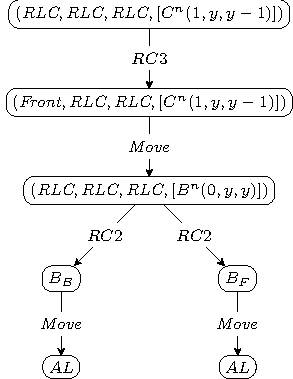
\includegraphics[scale=1]{figures/figCx12} 
	\end{center}
	where: \\
$ B_B = (\RLC, \RLC, \Back, [B^n(0, y, y)])$ and $ B_F = (\RLC, \RLC, \Front, [B^n(0, y, y)])$
and if $y=4$, $AL  = (\RLC, \RLC, \RLC, [L3^n(3, 0, 5)])$\\
otherwise $y > 4$, $AL = (\RLC, \RLC, \RLC, [A^n(y-1, 0, y+1)])$\\
Note that in both cases, the move from $B_B$ or $B_F$ leads to the same 
equivalence class of configurations: an $L3^n$ class when $y=4$ and 
an $A^n$ class otherwise. 
From Lemma~\ref{lemma:a}, the result holds for 
$x=1$ and $z = y-1$.

\item %y > 2 and z-y !=1->$A^n$
	If $2 < z < y-1$ (Recall that if $z=2$, since $x=1$, 
it is a $L2^n$ configuration), the moves are:\\
$succ_{RC3}~((\RLC, \RLC, \RLC, [C^n(1, y, z)]))$
$ = (\Front, \RLC, \RLC, [C^n(1, y, z)]), $\\
$ succ_{Move} (( \Front, \RLC, \RLC, [C^n(1, y, z)])$
$= (\RLC, \RLC, \RLC, [A^n(0, y, z+1)])$.\\
The last configuration is an $A^n$ configuration since $2<z<y-1$.
Similarly as above,  
%since the tree of root\\
%	$(\RLC, \RLC, \RLC, [A^n(x, 0, z)])$ is finite, 
the property results from Lemma~\ref{lemma:a}.
\end{itemize}
Finally, it results from the above cases that the tree
$\T(\RLC, \RLC, \RLC, [C^n(1, y, z)])$
 is finite for any $y, z$.


\begin{description}[parsep=0cm, itemsep=0cm, topsep=0cm]
\item[{\bf Induction step:} ] We now assume that the tree of root
  $(\RLC, \RLC, \RLC, [C^n(x, y, z)])$ is finite
  for any $y$, $z$, and prove that the same is true for 
  $\T(\RLC, \RLC, \RLC, [C^n(x+1, y, z)]$.
\end{description}  
\begin{itemize}[parsep=0cm, itemsep=0cm, topsep=0cm]
\item If $z=y-1$, the tree is%fait
	\begin{center}
	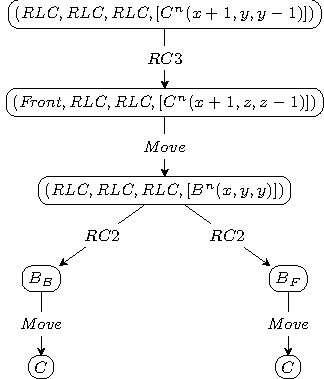
\includegraphics[scale=1]{figures/figCrec1} 
	\end{center}
	where\\
 	$\begin{array}{l c l}
B_B & = &(\RLC, \RLC, \Back, [B^n(x, y, y)])\\
B_F & = &(\RLC, \RLC, \Front, [B^n(x, y, y)]) \\
C & = &(\RLC, \RLC, \RLC, [C^n(x, y+1, y-1)])
\end{array}$\\
 	Thanks to the induction hypothesis, we can conclude that
  	the property holds in this case.
\item If $2 < z < y - 1$, applying the algorithm yields the movements: \\ 
$succ_{RC3}~((\RLC, \RLC, \RLC, [C^n(x+1, y, z)]))$
$ = (\Front, \RLC, \RLC, [C^n(x+1, y, z)]), $\\ 
$ succ_{Move} (( \Front, \RLC, \RLC, [C^n(x+1, y, z)])$ 
$= (\RLC, \RLC, \RLC, [C^n(x, y, z+1)])$.\\
The last configuration is a $C^n$ configuration since $2<z<y-1$, hence
the property holds from the induction hypothesis.
\end {itemize}
Finally all trees
$\T(\RLC, \RLC, \RLC, [C^n(x, y, z)])$ with
$0<x<z<y$ and $(x, z) \neq (1, 2)$ are finite.
% and thus from any $C^n$ configuration a legitimate configuration is
% finally reached, when $n \geq 10$ and $n, k$ are co-prime.
\end{proof}
%%%%%%%%%%%%%%%%%%%%%%%%%%%%%%%%%%%%%%%%%%%%%%%%%%%%%%
\begin{lemma}
\label{lemma:b}
The tree $\T(P)$ is finite for \\$P=(\RLC, \RLC, \RLC, [B^n(x, y, x), 
  x>0 \wedge x \neq y]).$
%$\forall c \in B^n, \texttt{conv}([B^n(x, y, y])=true$.

\end{lemma}
\begin{proof}
%For a simplification purpose this proof is done 
We handle two cases: $x>y$ and $x<y$.
% divisé en 2 un cas x < y et  x > y 

\noindent \textbf{Case $x>y$}:
%x <y pour tout y et ensuite pour tout x
  We first handle the subcases $y=0$ and $y=1$.
% a legitimate configuration
%  is eventually reached, then we show it for any $x, y$ such that
%  $x>y$.

%cas x=0 %y\geq 4
\begin{itemize}[parsep=0cm, itemsep=0cm, topsep=0cm]
\item When $y=0$, applying the algorithm yields the moves: \\
		\begin{center}
		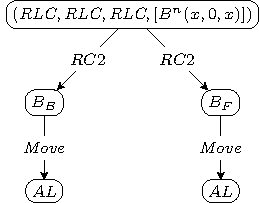
\includegraphics[scale=1]{figures/figBx0y4}
		\end{center}
	where \\
$\begin{array}{l c l}
	B_B & = &(\Back, \RLC, \RLC, [B^n(x, 0, x)])\\
	B_F & = &(\Front, \RLC, \RLC, [B^n(x, 0, x)]) 
\end{array}$\\
and if $x=4$, $AL =(\RLC, \RLC, \RLC, [L3^n(3, 0, 5)])$\\
otherwise $x>4$, $AL = (\RLC, \RLC, \RLC, [A^n(x-1, 0, x+1)])$\\
From $B^n$ configurations, where $y=0$, the moves lead to an $L3^n$ 
configurations when $x=4$, and to an $A^n$ configuration otherwise.
Hence,  from Lemma~\ref{lemma:a}, the property holds when $y=0$ for any $x$.
%cas x=1
\item When $y=1$, the tree representing the algorithm is the following:\\
		\begin{center}
		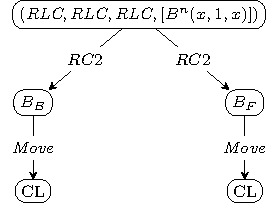
\includegraphics[scale=1]{figures/figBx1y3}
		\end{center}
		where\\
$\begin{array}{l c l}
	B_B & = &(\Back, \RLC, \RLC, [B^n(x, 1, x)])\\
	B_F & = &(\Front, \RLC, \RLC, [B^n(x, 1, x)])
\end{array}$\\
and if $x=3$, $CL =(\RLC, \RLC, \RLC, [L2^n(1, 4, 2)])$\\
otherwise $x>3$, $CL =(\RLC, \RLC, \RLC, [C^n(1, x+1, x-1)])$.\\
      Similarly as above there are two cases when $x=3$ or $x>3$.
      In the first case the moves reach $L2^n$ configurations, and in the
      second one to $C^n$ configurations.
      From Lemma~\ref{lemma:c}, the property holds when $y=1$ for any $x$.
\end{itemize}
	
\noindent
We now show the moves for any $x, y$ when $x>y>1$.  We need two
subcases when $x-1 = y$ and $x-1>y$.

\begin{itemize}[parsep=0cm, itemsep=0cm, topsep=0cm]
\item If $x-1=y$, the moves are:
	\begin{center}
	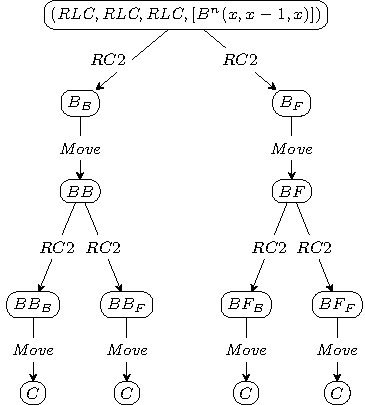
\includegraphics[scale=1]{figures/figBx+2y-1}
	\end{center}
	where\\
$\begin{array}{l c l}
	B_B & = &(\Back, \RLC, \RLC, [B^n(x, x-1, x)])\\
	B_F & = &(\Front, \RLC, \RLC, [B^n(x, x-1, x)])\\
	BB & = &(\RLC, \RLC, \RLC, [B^n(x+1, x-1, x-1)])\\
	BF & = &(\RLC, \RLC, \RLC, [B^n(x-1, x-1, x+1)])\\
		BB_B & = &(\RLC, \RLC, \Back, [B^n(x+1, x-1, x-1)])\\
		BB_F& = &(\RLC, \RLC, \Front, [B^n(x+1, x-1, x-1)])\\
		BF_B & = &(\RLC, \Back, \RLC, [B^n(x-1, x-1, x+1)])\\
		BF_F& = &(\RLC, \Front, \RLC, [B^n(x-1, x-1, x+1)])\\%%%
	C & = &(\RLC, \RLC, \RLC, [C^n(x-2, x+1, x)])\\
\end{array}$

\smallskip The property holds in this case, thanks to Lemma~\ref{lemma:c}.
\item If $x-1>y$, and $y>1$ the tree is:\\
	\begin{center}
	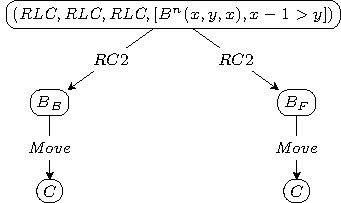
\includegraphics[scale=1]{figures/figBx+2y-1?}
	\end{center}
	where\\
		$\begin{array}{l c l}
	B_B & = &(\Back, \RLC, \RLC, [B^n(x, y, x)])\\
	B_F & = &(\Front, \RLC, \RLC, [B^n(x, y, x)])\\
	C & = &(\RLC, $ $\RLC, \RLC, [C^n(x+1, y, x-1)])	
		\end{array}$\\
and Lemma~\ref{lemma:c} entails the result. 
\end{itemize}
Hence,  $\T(\RLC, \RLC, \RLC, [B^n(x, y, x), x>y]))$ is finite.

%\medskip 
\noindent \textbf{Case $x<y$}: 
%x >y pour tout x et ensuite pour tout y
%We show that from any configuration of type $B$ 
%for any $x, y$ such that $x<y$ a legitimate configuration is eventually reached.
We handle two subcases when $y>x+1$ and $y=x+1$.

\begin{itemize}[parsep=0cm, itemsep=0cm, topsep=0cm] 
	\item If $x+1<y$, then the moves are:\\
		\begin{center}
		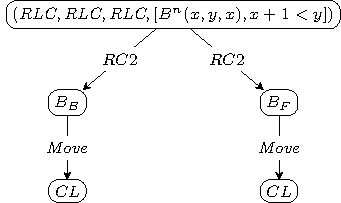
\includegraphics[scale=1]{figures/figBx1}
		\end{center}
	where\\
$\begin{array}{l c l}
B_B & = &(\Back, \RLC, \RLC, [B^n(x, y, x), x+1<y)])\\
B_F & = &(\Front, \RLC, \RLC, [B^n(x, y, x), x+1<y)
\end{array}$\\
and if $x=1$\\
$\begin{array}{l c l}
CL & = &(\RLC, $ $\RLC, \RLC, [L1^n(2, y, 0)])
\end{array}$\\
otherwise ($x>1$):\\
$\begin{array}{l c l}	
CL & = &(\RLC, \RLC, \RLC, [C^n(x-1, y, x+1)])
\end{array}$\\
When $x=1$ the moves lead to $L1^n$ configurations and 
to $C^n$ configurations otherwise.
Hence, again thanks to Lemma~\ref{lemma:c}, 
the property holds for any $x, y$ when $x+1<y$.

\smallskip
\item If $x+1=y$, the tree is:\\
		\begin{center}
		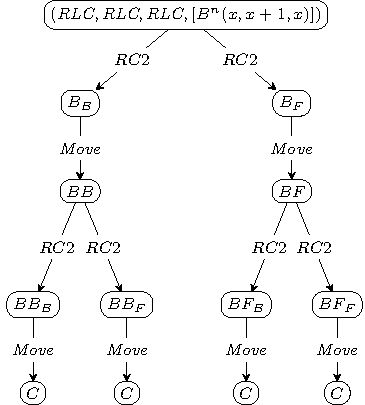
\includegraphics[scale=1]{figures/figBx+1y}
		\end{center}
	
		where\\
$\begin{array}{l c l}
B_B & = & (\Back, \RLC, \RLC, [B^n(x, x+1, x)])\\
B_F  & = & (\Front, \RLC, \RLC, [B^n(x, x+1, x)])\\
BB  & = & (\RLC, \RLC, \RLC, [B^n(x+1, x+1, x-1)])\\
BF & = &  (\RLC, \RLC, \RLC, [B^n(x-1, x+1, x+1)])\\
BB_B  & = & (\RLC, \Back, \RLC, [B^n(x+1, x+1, x-1)])\\
BB_F & = & (\RLC, \Front, \RLC, [B^n(x+1, x+1, x-1)])\\
BF_B & = & (\RLC, \RLC, \Back, [B^n(x-1, x+1, x+1)])\\
BF_F  & = & (\RLC, \RLC, \Front, [B^n(x-1, x+1, x+1)])\\
C & = & (\RLC, \RLC, \RLC, [C^n(x, x+2, x-1)])\\
\end{array}$\\

Since $\T(\RLC, \RLC, \RLC, [C^n(x, y, z)])$ is
finite (by Lemma~\ref{lemma:c}), the property holds.
\end{itemize}
Finally the trees
$\T(\RLC, \RLC, \RLC[B^n(x, y, x), x<y])$
are also finite, which concludes the proof.

%Hence,  $\T(\RLC, \RLC, \RLC, [B^n(x, y, x)])$ is finite.
\end{proof}

%Now the remaining lemmas are easier to prove.
\begin{lemma}
\label{lemma:e}
The tree $\T(P)$ is finite for $P=(\RLC, \RLC, \RLC, [E^n(0, 1, z)]).$
\end{lemma}

\begin{proof}
In the case of $E^n$ configurations, we have:
%\paragraph{Configurations of type $E$}
\begin{center}
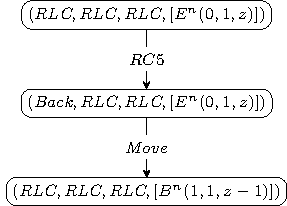
\includegraphics[scale=1]{figures/figE}
\end{center}
and the result holds thanks to Lemma~\ref{lemma:b}.
\end{proof}


\begin{lemma}
\label{lemma:d}
The tree $\T(P)$ is finite for $P=(\RLC, \RLC, \RLC, [D^n(0, 0, z)]).$
\end{lemma}
%\paragraph{Configurations of type $D$}

\begin{proof}
  From a $D^n$ configuration, it is also possible to schedule two
  robots with their respective planned moves. The various cases lead
  to either an $E^n$ configuration with or without a pending
  movement, or a $B^n$ configuration:\\
\begin{center}
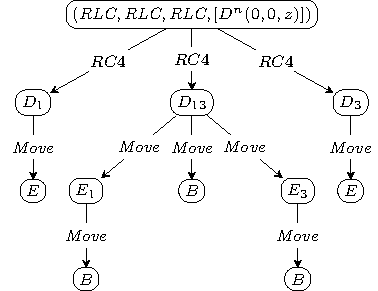
\includegraphics[scale=1]{figures/figD}%%%%%%%%%%%%%%%%%%%%%%%%%%%%%%%%%%%%%%%%%
\end{center}
	where\\
$\begin{array}{l c l}
D_1 & = &(\Back, \RLC, \RLC, [D^n(0, 0, z)])\\
D_{13} & = &(\Back, \RLC, \Back, [D^n(0, 0, z)])\\
D_3 & = &(\RLC, \RLC, \Back, [D^n(0, 0, z)])\\
E & = &(\RLC, \RLC, \RLC, [E^n(0, 1, z-1)])\\
E_1 & = &(\RLC, \RLC, \Back, [E^n(1, 0, z-1)])\\
E_3 & = &(\Back, \RLC, \RLC, [E^n(0, 1, z-1)])\\
B & = &(\RLC, \RLC, \RLC, [B^n(1, 1, z-2)])\\
\end{array}$\\
and the result holds from the previous lemmas~\ref{lemma:b} and~\ref{lemma:e}.
\end{proof}

%The proofs of the four other lemmas are similar and are given in
%Appendix.  
Together these lemmas imply Theorem~\ref{th:conv}. Finally, 
Theorems~\ref{th:legit} and~\ref{th:conv} give the result for
perpetual exploration. Moreover, since all reachable configurations
from any of the initial configurations are tower-free, the
\emph{Exclusivity} property follows (recall that the
\emph{No\_collision} property implies the \emph{No\_switch} property
in the asynchronous case as mentioned in
Section~\ref{subsub:perpexp}).  This concludes the correctness proof
of the algorithm.
	
		